\documentclass[]{article}
\usepackage{graphicx}
\usepackage{float}

%opening
\title{Software Design Document}
\author{Ayman, Belal, Khaled, Karim, Mostafa}

\begin{document}

\maketitle

\section{Introduction}
\subsection{Purpose}
This software design document describes the architecture and system design of (ADwytee)


\subsection{Scope}
Our project will target mainly two users (Normal User, Pharmacy)
\newline
\newline
\textbf{\underline{Normal User}}
\newline
\newline
1-He will be able to search for a certain medicine on our web application and our database server will provide him with the location of the nearest pharmacies in ascending order
\newline
2-He will be able to track certain medicine and the server will notify him whenever it's available
\newline
3-He will be able to set schedule and the server will notify and provide him with the available pharmacies
\newline
4-He will be able to view alternatives in ascending order according to the highest recommendation
\newline
5-He will be able to print a card containing his unique key
\newline
6-Every user will have a patient profile for view only
\newline
\newline
\textbf{\underline{Pharmacy}}
\newline
\newline
1-Registered pharmacies will be able to provide users with their location and brief details about the pharmacy
\newline
2-It will provide the server with available medicines real time
\newline
3-It will be able to add or remove medicine from its database
\newline
4-It will be able to add new medicine to the database and provide brief details about it
\newline
5-It will be able to edit medicine info
\newline
6-It will be able to set medicines alternatives
\newline
7-It will be able to edit the patient profile using the unique key of the patient
\newline
8-It will be able to bind a patient using his unique key


\subsection{Overview}
This document will go over the design of various aspects of the project including architectural, software components, interface, database design and steps on how the users will interact with the system 


\section{System Overview}
The system will depends mainly on our API server where it will be responsible for the connections with the database server and the database interactions in order to maintain this process we have to separate the API section from the web application server provider   

\section{System Architecture}
\subsection{Architectural Design}

\begin{figure}[H]
\centering
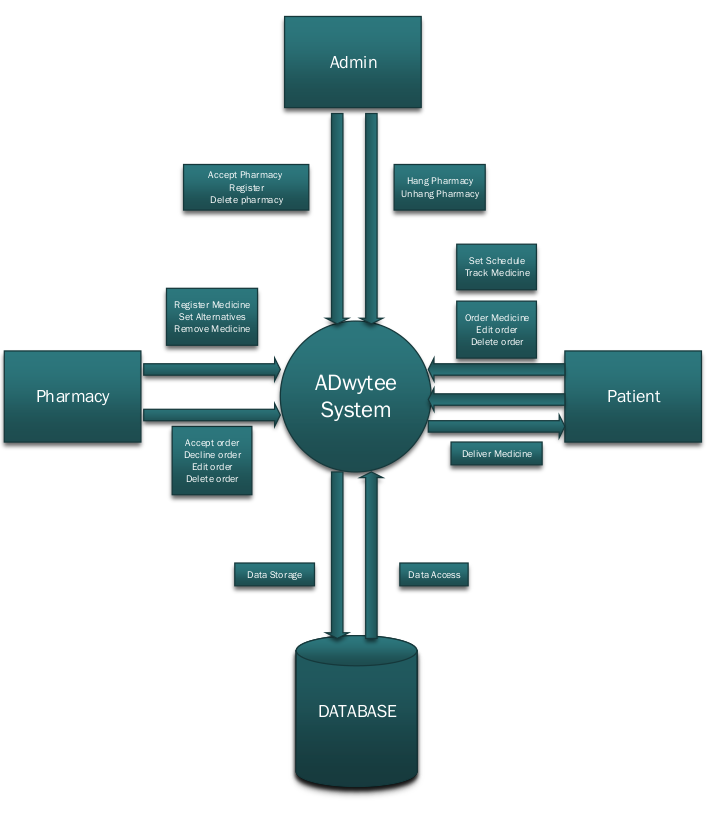
\includegraphics[scale=0.4]{./block}
\caption{Block Diagram}
\end{figure}


\subsection{Decomposition Description}
...


\subsection{Design Rationale}
...


\section{Data Design}
\subsection{Data Description}
The major data or system entities are stored with MySQL database using PHP Scripts installed on the local web server.

\begin{figure}[H]

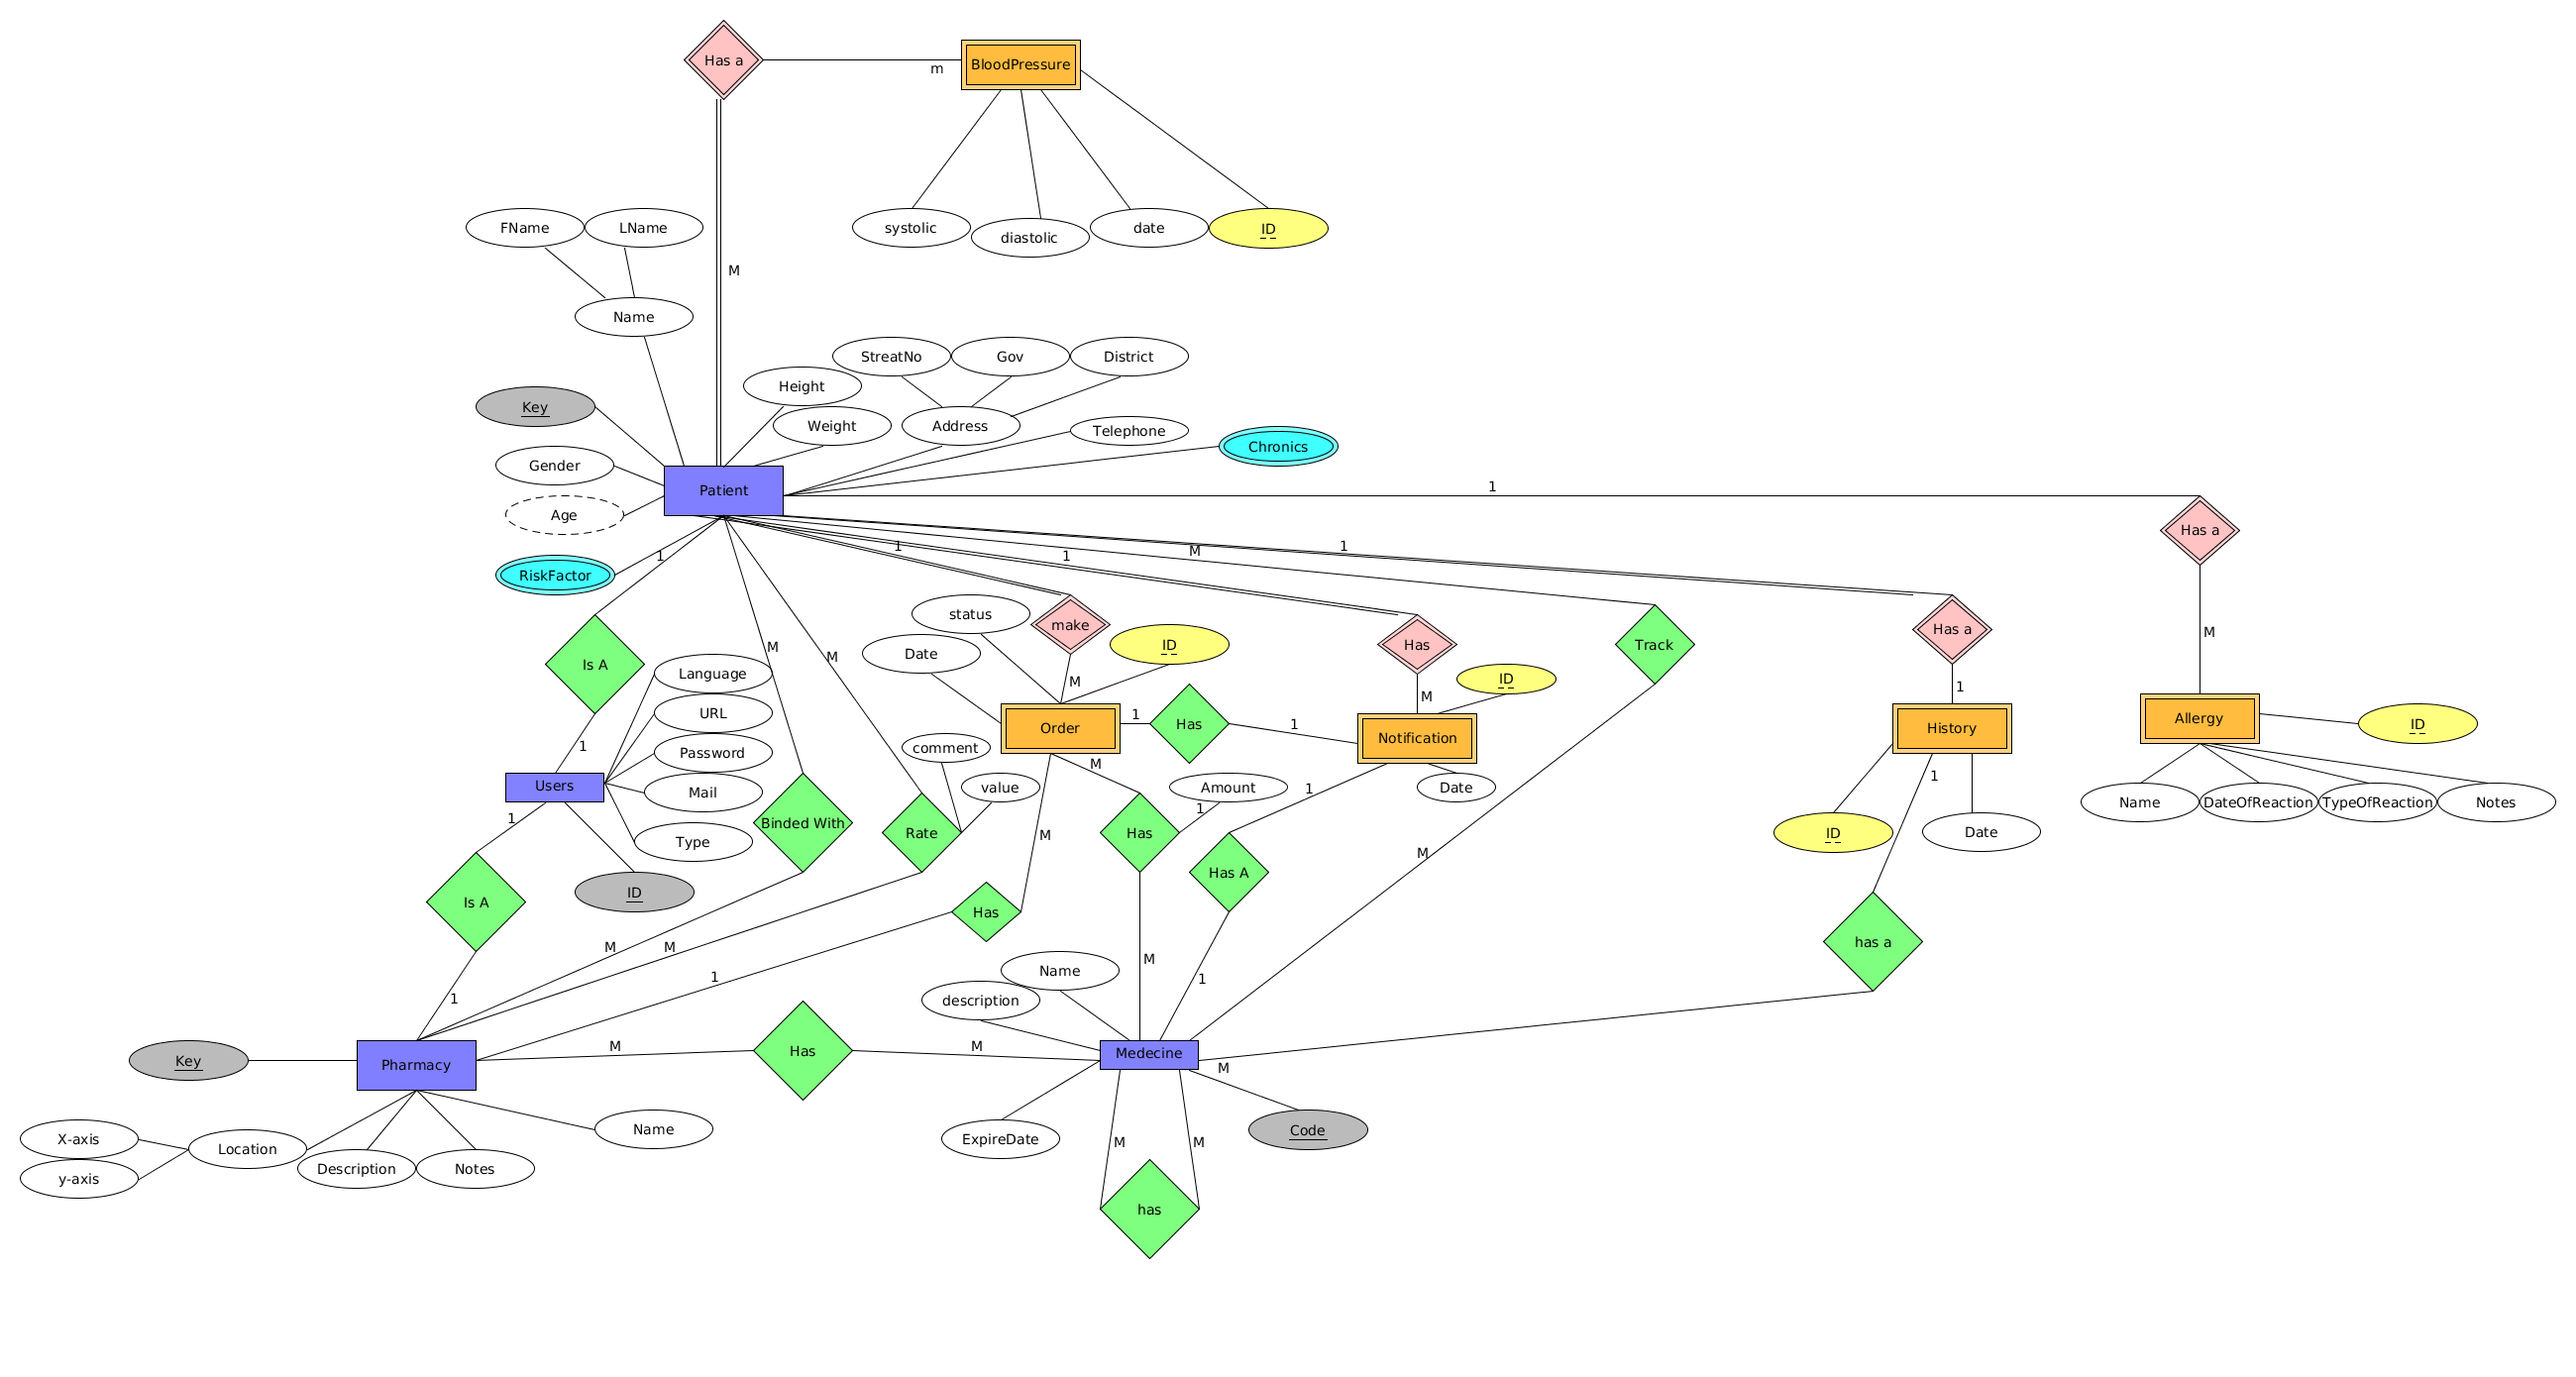
\includegraphics[scale=0.18]{./database/Erd}
\caption{ERD}
\end{figure}

\begin{figure}[H]
\centering
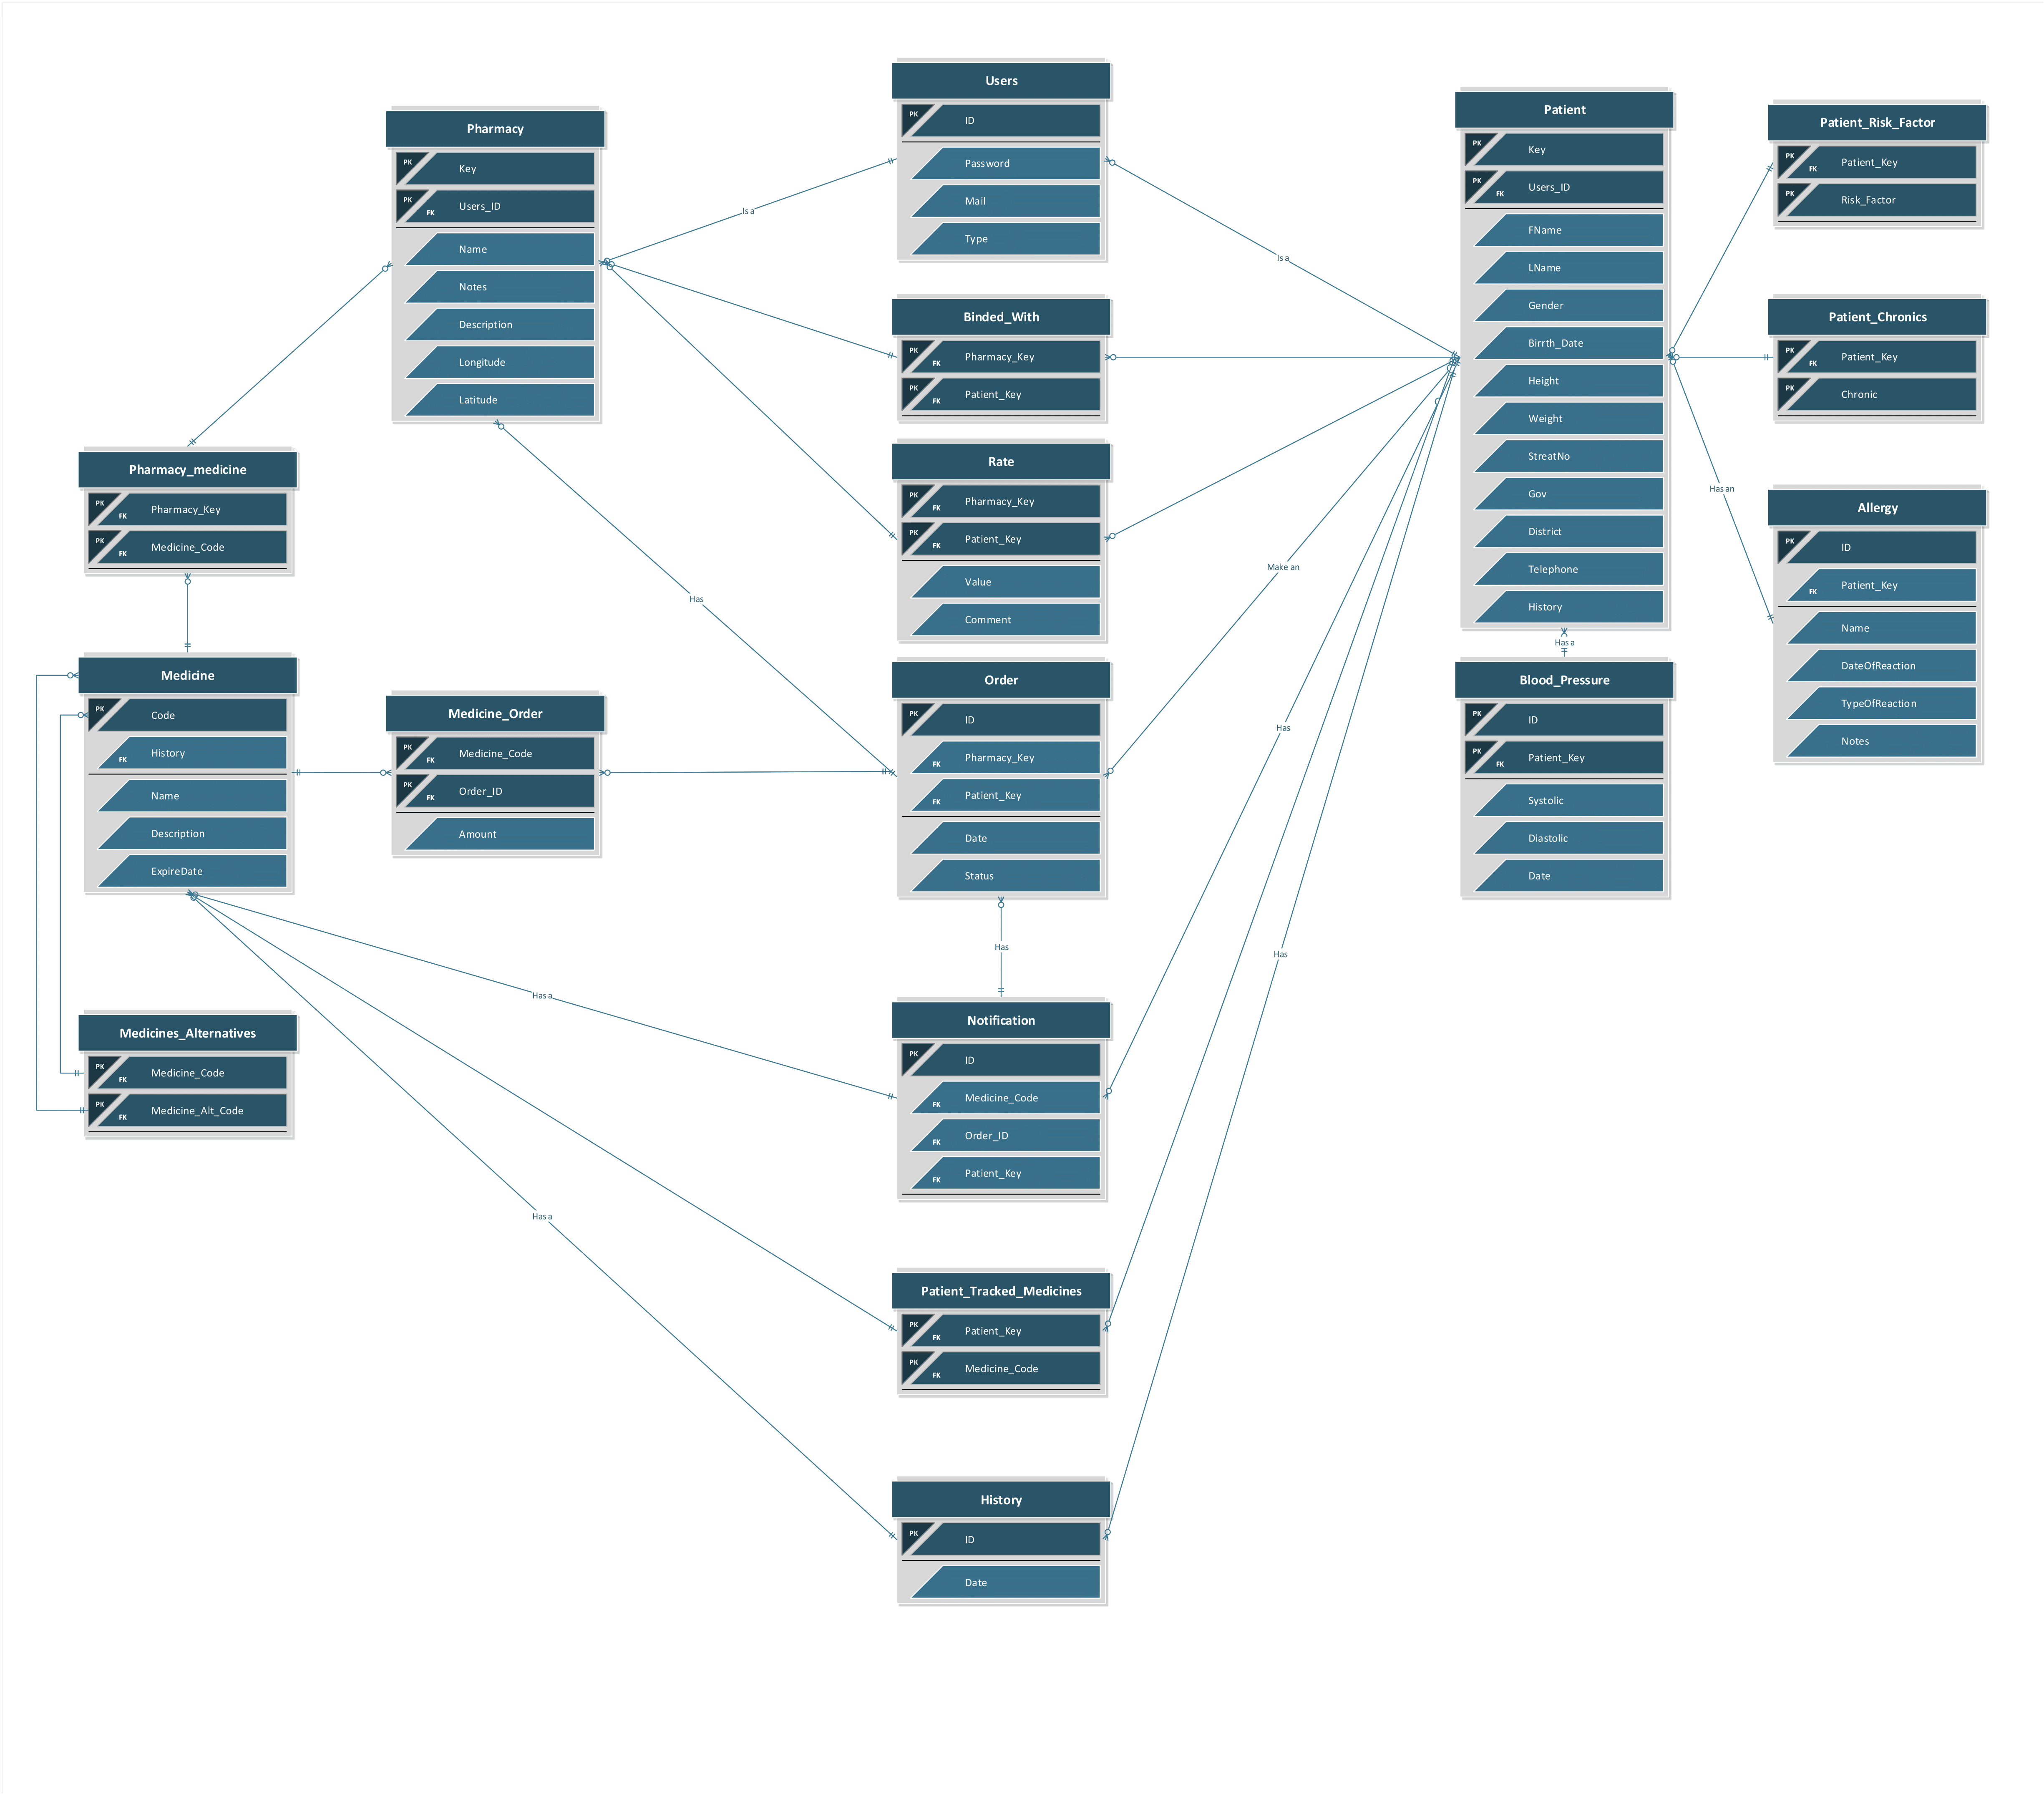
\includegraphics[scale=0.1]{./database/DatabaseTables}
\caption{Database Tables}
\end{figure}

\subsection {Data Dictionary}
...

\section{Component Design}
...


\section{Humnan Interface Design}

\subsection {Overview of User Interface}
On the home page user will be able to search for certain medicine, the system will try to predict his location
\newline
On failure the website will ask him to enter it manually
\newline
The results will be displayed on the next page (Results page) it will provide him with location of the pharmacies that have medicines, the user will be able to select either medicine or the pharmacy providing it.
\newline
Upon selecting the medicine he will be able to know it's info and the alternatives to that medicine.
\newline
Upon selecting the pharmacy he will get info about it and it's location on map.
\newline
\newline
Registered user will be able to set a schedule from a drop down menu or even track a medicine.
\newline
Upon tracking a medicine the website will notify him whenever the medicine is available.
\newline
\newline
Registered pharmacy will choose either manage medicines (add or remove), bind a user, view and edit patient profile from the drop down menu
\newline

\subsection {Screen Images}

\begin{figure}[H]
\centering
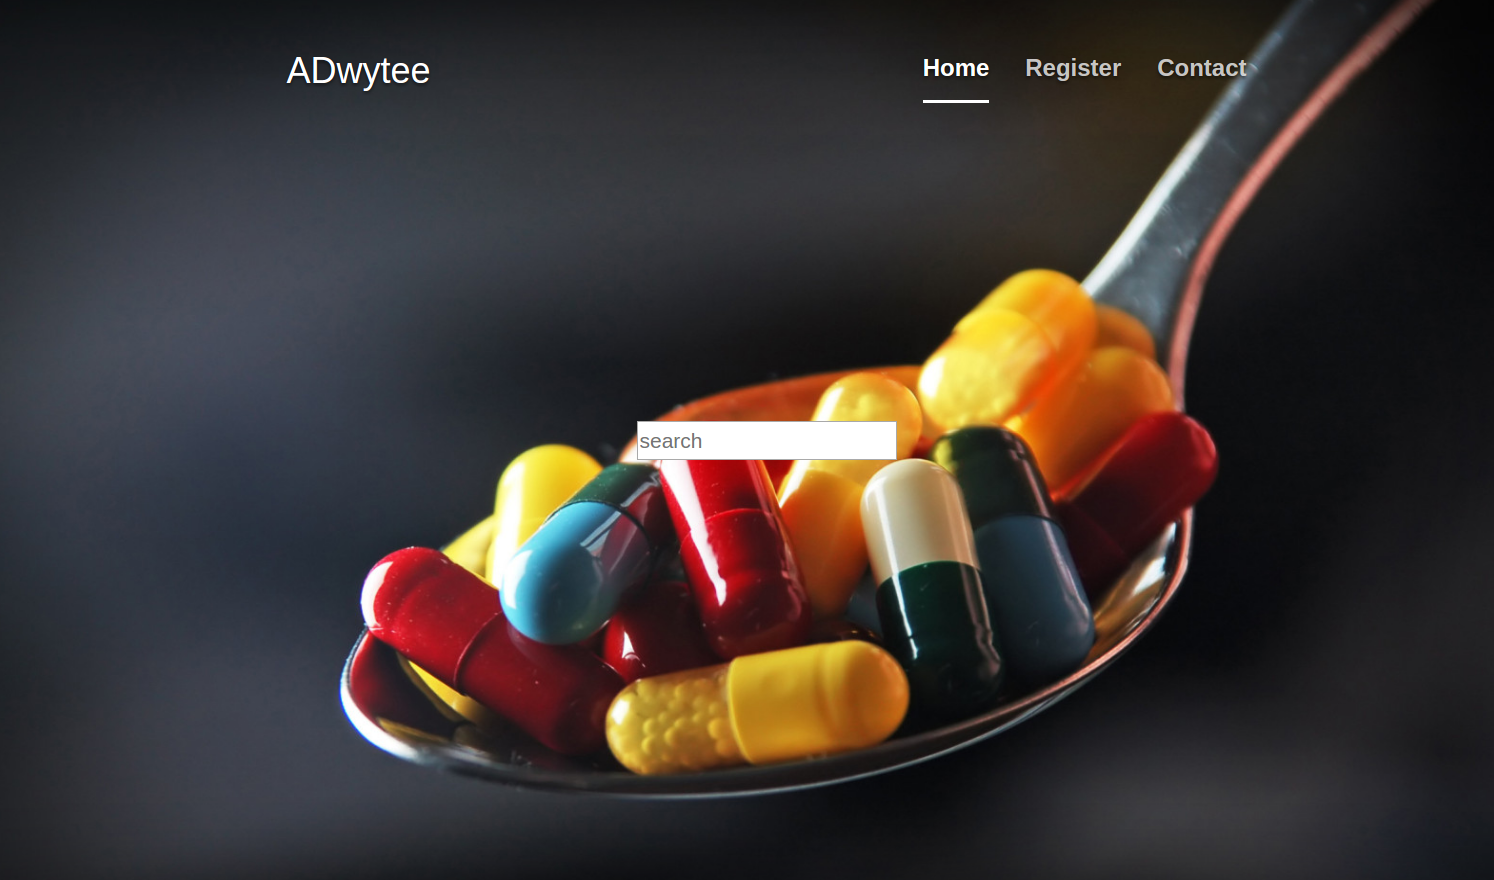
\includegraphics[scale=0.18]{./Home}
\end{figure}


\subsection {Screen Objects and Actions}
The Home page provides you with links to the other pages within the web application and displays an overview of what is expected of the application and provides a search bar to search for a specific medicine.


\section{Requirements Matrix}
...


\section{APPENDICES}
...

\section {References}
\bibliographystyle{IEEEtranS}

\bibliography{dissertationbib}

\end{document}
\grid